\input{./_path-to-root.ltx}
\documentclass[\PathToRoot/\ProjectName]{subfiles}
\whenstandalone{\externaldocument{\PathToRoot/\ProjectName}}

\begin{document}

\begin{figure}[H]
  \centering
  \caption{General equilibrium policy comparison in HANK-SAM model}
  \whenintegrated{\label{fig:HANK_IRFs}} 
  \noindent\begin{minipage}{\textwidth}
    \centering
    \begin{subfigure}[b]{.30\linewidth}
      \centering
      % Original path: \PathToRoot/Code/HA-Models/FromPandemicCode/Figures/HANK_transfer_irf
      \includegraphics[width=\linewidth]{\PathToRoot/images/HANK_transfer_IRF}
      \caption{Stimulus check IRF}
      \whenintegrated{\label{fig:hank_stimulus_irf}} 
    \end{subfigure}
    %
    \begin{subfigure}[b]{.30\linewidth}
      \centering
      % Original path: \PathToRoot/Code/HA-Models/FromPandemicCode/Figures/HANK_UI_irf
      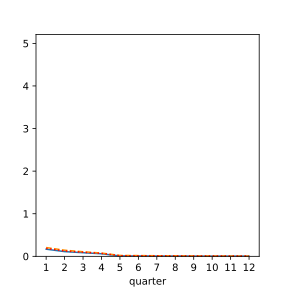
\includegraphics[width=\linewidth]{\PathToRoot/images/HANK_UI_IRF}
      \caption{UI extension IRF}
      \whenintegrated{\label{fig:hank_UI_irf}} 
    \end{subfigure}
    %
    \begin{subfigure}[b]{.30\linewidth}
      \centering
      % Original path: \PathToRoot/Code/HA-Models/FromPandemicCode/Figures/HANK_tax_irf
      \includegraphics[width=\linewidth]{\PathToRoot/images/HANK_tax_IRF}
      \caption{Payroll tax cut IRF}
      \whenintegrated{\label{fig:hank_tax_irf}} 
    \end{subfigure}
    \\[1em]
    \begin{subfigure}[b]{.30\linewidth}
      \centering
      % Original path: \PathToRoot/Code/HA-Models/FromPandemicCode/Figures/HANK_transfer_multiplier
      \includegraphics[width=\linewidth]{\PathToRoot/images/HANK_transfer_multiplier}
      \caption{Stimulus check multiplier}
      \whenintegrated{\label{fig:HANK_transfer_multiplier}} 
    \end{subfigure}
    %
    \begin{subfigure}[b]{.30\linewidth}
      \centering
      % Original path: \PathToRoot/Code/HA-Models/FromPandemicCode/Figures/HANK_UI_multiplier
      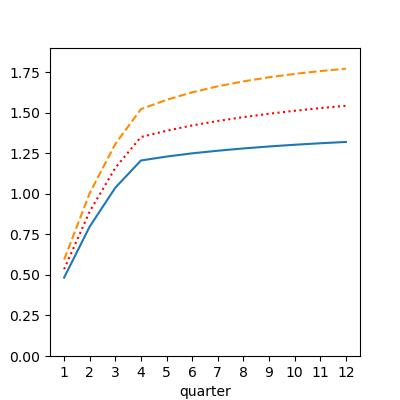
\includegraphics[width=\linewidth]{\PathToRoot/images/HANK_UI_multiplier}
      \caption{UI extension multiplier}
      \whenintegrated{\label{fig:HANK_UI_multiplier}} 
    \end{subfigure}
    %
    \begin{subfigure}[b]{.30\linewidth}
      \centering
      % Original path: \PathToRoot/Code/HA-Models/FromPandemicCode/Figures/HANK_tax_multiplier
      \includegraphics[width=\linewidth]{\PathToRoot/images/HANK_tax_multiplier}
      \caption{Payroll tax cut multiplier}
      \whenintegrated{\label{fig:HANK_tax_multiplier}} 
    \end{subfigure}
  \end{minipage}
\end{figure}
\noindent\parbox{\textwidth}{\footnotesize
  \textbf{Note}: This figure presents general equilibrium results from the HANK-SAM model (Section~\ref{sec:hank}).
  Subfigures~(a)-(c) show consumption impulse responses under three monetary policy rules:
  active Taylor rule, fixed nominal rate (ZLB), and fixed real rate.
  Subfigures~(d)-(f) show corresponding cumulative multipliers over time.
  The general equilibrium framework generates multipliers through an intertemporal Keynesian cross mechanism,
  particularly pronounced when monetary policy is passive.
  Results validate the partial equilibrium findings that UI extensions achieve the highest multipliers
  across all policy environments.
}

\vspace{1em}  % Add space after figure

% Smart bibliography: Only include bibliography if standalone AND has citations
\smartbib

\end{document}
